%!TEX root = paper.tex

\section{Introduction}
\label{sec:intro}


Statistical inference is an important technique to express hypothesis and
reason about data in data analytical tasks.  
Today, many big data applications are based on
statistical inference.
Examples include topic modeling \cite{blei2003latent,Titov2008a},
sentiment analysis \cite{Titov2008b, Jo2011,tsm}, spam filtering \cite{spam}, to name a few.


One of most critical steps of statistical inference is to construct a
\emph{statistical model} to formally represent the underlying statistical
inference task \cite{cox}.  The development of a statistical
model is never trivial because a domain user may have to devise and
implement many  different models before finding a promising one for a specific
task.  Currently, most scalable machine learning libraries (e.g. MLlib \cite{mllib}) only
contain standard models like support vector machine, linear regression, latent
Dirichlet allocation (LDA) \cite{blei2003latent}, etc.  
To carry out statistical inference on
customized models with big data, the user has to implement her own models and
inference codes on a distributed framework like Apache Spark
\cite{Zaharia:2010:SCC:1863103.1863113} and Hadoop \cite{hadoop}.

Developing inference code requires extensive knowledge in both statistical
inference and programming techniques in distributed frameworks.  Moreover,
model definitions, inference algorithms, and data processing tasks are all
mixed up in the resulting code, making it hard to debug and reason about.  For
even a slight alteration to the model in quest of the most promising one, the
model designer will have to re-derive the formulas and re-implement the
inference codes, which is tedious and error-prone. 

In this paper, we present InferSpark, a \emph{probabilistic programming
framework} on top of Spark.  Probabilistic programming is an emerging
paradigm that allows statistician and domain users to succinctly express a model
definition within a host programming language and transfers the burden of
implementing the inference algorithm from the user to the compilers and
runtime systems \cite{pp}.  For example, Infer.NET \cite{InferNET14} is a
probabilistic programming framework that extends C\#.  The user can express,
say, a Bayesian network in C\# and the compiler will generate code to perform
inference on it. Such code could be as efficient as the implementation of
the same inference algorithm carefully optimized by
an experienced programmer.

So far, the emphasis of probabilistic programming has been put on the
expressiveness of the languages and the development of efficient inference
algorithms (e.g., variational message passing \cite{vmp}, Gibbs sampling \cite{gibbs},
Metropolis-Hastings sampling \cite{mh}) to handle a wider range of statistical
models.  The issue of scaling out these frameworks, however, has not been
addressed.  For example, Infer.NET only works on a single machine.  
When we tried to use Infer.NET to train an LDA model of 96 topics and 9040-word
vocabulary on only 3\% of Wikipedia articles, the actual memory
requirement has already exceeded 512GB, the maximum memory of most commodity
servers today.
%Frequent swapping makes each iteration take xxx hrs
%(still running, > 2 hr). Infer .NET deals with the scaling problem by
%splitting the whole dataset into chunks that fit in memory and iteratively
%load and process the chunks. Using the batched training, each iteration still
%takes over 21 minutes.  
The goal of InferSpark is thus to bring 
probabilistic programming to Spark, a predominant distributed data
analytic platform, for carrying out statistical inference at scale. 
The InferSpark project consists of two parts:

\begin{packed_enum}
	\item {\bf Extending Scala to support probabilistic programming}

	Spark is implemented in Scala due to its functional nature.
The fact that both preprocessing and post-processing can be 
included in one Scala program substantially eases the development process.
	In InferSpark,
	we extend Scala with probabilistic programming constructs to leverage its
	functional features.  Carrying out statistical inference with InferSpark
	is simple and intuitive, and implicitly enjoys the distributed computing
	capability brought by Spark.  As an example, the LDA statistical model was
	implemented using 503 lines of Scala code in MLlib (excluding comments,
	javadocs, blank lines, and utilities of MLlib).  With InferSpark, we could
	implement that using only 7 lines of Scala code (see
	\figref{fig:intro_lda_def}). 
	

	\item {\bf Building an InferSpark compiler and a runtime system}
		
	InferSpark compiles InferSpark models into Scala classes
	and objects that implement the inference algorithms with a set of API. The
	user can call the API from their Scala programs to specify the input
	(observed) data and query about the model (e.g. compute the expectation of
	some random variables or retrieve the parameters of the posterior
	distributions).
		
\end{packed_enum}


\begin{figure}
\begin{lstlisting}
@Model
class LDA(K: Long, V: Long, alpha: Double, beta: Double){
	val phi = (0L until K).map{_ => Dirichlet(beta, K)}
	val theta = ?.map{_ => Dirichlet(alpha, K)}
	val z = theta.map{theta => ?.map{_ => Categorical(theta)}}
	val x = z.map{_.map{z => Categorical(phi(z))}}
}
\end{lstlisting}
\label{fig:intro_lda_def}
\caption{Definition of Latent Dirichlet Allocation Model}
\end{figure}

Currently, InferSpark supports Bayesian network models. Bayesian network
is a major branch of probabilistic graphical model and it has already covered
models like naive Bayes, LDA, TSM \cite{tsm}, etc.  The goal of this paper is to
describe the workflow, architecture, and Bayesian network implementation of
InferSpark.  We will open-source InferSpark and support other models (e.g.,
Markov networks) afterwards.  

To the best of our knowledge, InferSpark is the first endeavor to bring 
probabilistic programming into the (big) data engineering domain.
Efforts like MLI \cite{mli} and SystemML \cite{systemml} all aim 
at easing the difficulty of developing \emph{distributed machine learning techniques} 
(e.g., stochastic gradient descent (SGD)).
InferSpark aims at easing the complexity of developing \emph{custom statistical models}, 
with statistician, data scientists, and machine learning researchers as the target users.
This paper presents the following technical contributions of InferSpark so far.
\begin{packed_enum}
\item We present the extension of Scala's syntax that can express various sophisticated 
Bayesian network models with ease.
\item We present the details of compiling and executing an InferSpark program on Spark.
That includes the mechanism of automatic generating efficient inference codes that 
include checkpointing (to avoid long lineage), proper timing of caching and 
anti-caching (to improve efficiency under memory constraint),
 and partitioning (to avoid unnecessary replication and shuffling).
\item We present an empirical study that shows InferSpark can enable 
statistical inference on both customized and standard models at scale.
\end{packed_enum}

%
%For example, Bayesian inference algorithms are mostly iterative serial
%algorithms. When implementing them on Spark, we have to identify the
%parallelizable parts without violating the correctness of the algorithms and
%also adapt them to the computation model.
%% (\ZY{not the problem of
%%functional style. when updating a vertex $v$, $v$ needs to pull message from
%%neighbours $u$, and before the neighbours can return the message, they may
%%need to pull messages from their neighbours.
%%This translates to either 2 ``aggregate'' and 2
%%``join'', or 1 and 1 with cached message in GraphX.}). 
%Furthermore, 
%Spark is efficient for iterative machine learning algorithms 
%that does not modify the in-memory RDD (e.g., Stochastic Gradient Descent in MLlib). 
%%
%%because the data can reside in the memory as RDD,
%%
%%as long as the
%%data reside in the memory, especially for algorithms 
%Statistical inference algorithms like VMP \cite{vmp}, however, 
%require iteratively update the RDD.
%Therefore, the implementation requires persisting  the 
%intermediate results before the first action of the next
%iteration to avoid unnecessary shuffling and 
%unpersisting afterwards so that
%the memory consumption does not increase linearly with the number of iterations.
%It is also necessary to periodically checkpoint the RDD to avoid long lineage,
%which could overflow the memory and crash the program. \KZ{One might ask,
%is Spark the right choice to implement PP on, if there's so much difference
%between the intrinsic computation model of Spark and VMP?}

The remainder of this paper is organized as follows: 
Section \ref{sec:background} presents the essential background for this paper.
Section \ref{sec:framework} then gives an overview of InferSpark.
Section \ref{sec:implementation} gives the implementation details of InferSpark.
Section \ref{sec:eval} presents an evaluation study of the current version of InferSpark.
Section \ref{sec:related} discusses related work 
and Section \ref{sec:conclusion} contains our concluding remarks.



%Proper persisting,
%unpersisting and checkpointing is crucial to such iterative programs but are
%not easy to do in GraphX because not all combinations will work as it should.
%

%The iterative nature of 
%inference algorithms is also a challenge because long running iterative
%programs on Spark could easily take excessively long to finish or even crash
%if the intermediate results are not properly persisted, unpersisted or
%checkpointed. 
%We also have to deal with various compatibility issues among
%Spark, scala and JVM because our framework also makes use of several advanced
%features of scala.


%Despite availability of various statistical models, new models are constantly
%being proposed to adapt to different characteristics of the data. In the case
%of topic modeling, LDA is a widely used model but may still be outperformed
%by other topic models when used on different datasets. 
%
%
%Nowadays, many new applications often
%call for various customized models, such as topic modelling
%
%The naive Bayes model is a simple classification model that has been
%successfully used in spam filtering and medical diagnosis.  In spam filtering,
%bag-of-word features are typically used. Each email is viewed as a set of words
%that appear at least once in it. The naive Bayes model assumes that the
%occurence of each word is independent and the probability of a spam email is
%simply the product of the probabilities of being a spam conditioned on each
%word. The conditional probabilities are inferred from a number of labeled
%emails. Given a new email, the trained model can give a probability of the
%email being spam.  When the probability is higher than some threshold, the
%email can be identified as a spam. Assigning zero probability to missing words
%in the training data could degrade the performance because any new email
%containing the missing word is assigned probability zero. Laplacian smoothing
%is used in such models to avoid giving zero probability to missing words in the
%training data.  Alternatively, adding a Beta prior to the parameters and
%performing Bayesian inference with the training data is equivalent to the
%laplacian smoothing. Besides the naive Bayes model, it is also possible use
%other classification models such as logistic regression and support vector
%machine.
%
%The latent Dirichlet allocation is a popular topic model. It is widely used to
%summarize topics from a lot of documents and to tag the documents with the
%topics. The LDA model describes a probabilitic generative process of the
%documents. With the documents as input, inference algorithm calculates the
%poseterior distribution of the parameters of the LDA model and generate lists
%of representative words for the topics. For example, it can produce lists of
%keywords for paper abstracts when trained with scientific papers. Meanwhile,
%from the posterior distribution computed by the inference algorithm, the most
%probable topics are assigned to the document.  The result can be used to
%categorize the papers according to their topics, saving a lot of manual labour.
%
%The LDA model is not the only choice of topic models. For example, the
%Sentence LDA model uses a sentence-level topic instead of per-word topic to
%capture the property that words in a sentence tend to share the same topic.
%The Dirichlet compound multinomial LDA \cite{Doyle2009} model uses differnt
%topic-word distributions in each document instead of a global one to account
%for the burstiness in a corpus.
%
%In online shopping sites, the users may express positive or negative feelings
%toward different aspects of a product (e.g. price, quality) in their comments,
%but it usually takes a lot of time for readers to obtain the information.
%Online shopping sites can use the sentiment and aspect information to collect
%feedbacks for improvement and allow users to quickly evaluate the products
%according to the senti-aspect keywords of others' comments. A lot of models
%such as the Topic Sentiment Model \cite{Mei2007}, the Multi-Grain LDA model
%\cite{Titov2008a}, the Aspect and Sentiment Unification Model \cite{Jo2011}
%and etc. are constantly proposed to extract the sentiment and aspect
%information from the user reviews.
%
%Despite avaliability of various statistical models, new models are constantly
%being proposed to adapt to different characteristics of the data. In the case
%of topic modelling, LDA is a widely used model but may still be outperformed
%by other topic models when used on different datasets. The development of
%models is not a easy task because the user may have to try differnt
%possibilities. For even a slight alteration to the existing model, the
%designer will have to re-derive the formulas and re-implement the inference
%algorithms.  Probabilistic programming allows the designer to simply write the
%model definition using a succint language and leave the inference task to the
%system, which offloads the burden of implementation and makes it much easier
%to evaluate a new model.
%
%Currently, most machine learning libraries (e.g. MLLib) only contain standard
%models like support vector machine, linear regression, latent Dirichlet
%allocation (LDA) and etc. To perform inference on customized models, the user
%has to implement his own algorithms instead of the off-the-shelf algorithms
%provided by the ML libraries. Developing inference code requires extensive
%knowledge in both Bayesian inference and programming techniques in distributed
%frameworks.  Moreover, model definition, inference algorithm and unrelated
%code are all mixed up in the resulting code, making it hard to debug and
%resaon about.

%\begin{figure*}[!th]
%	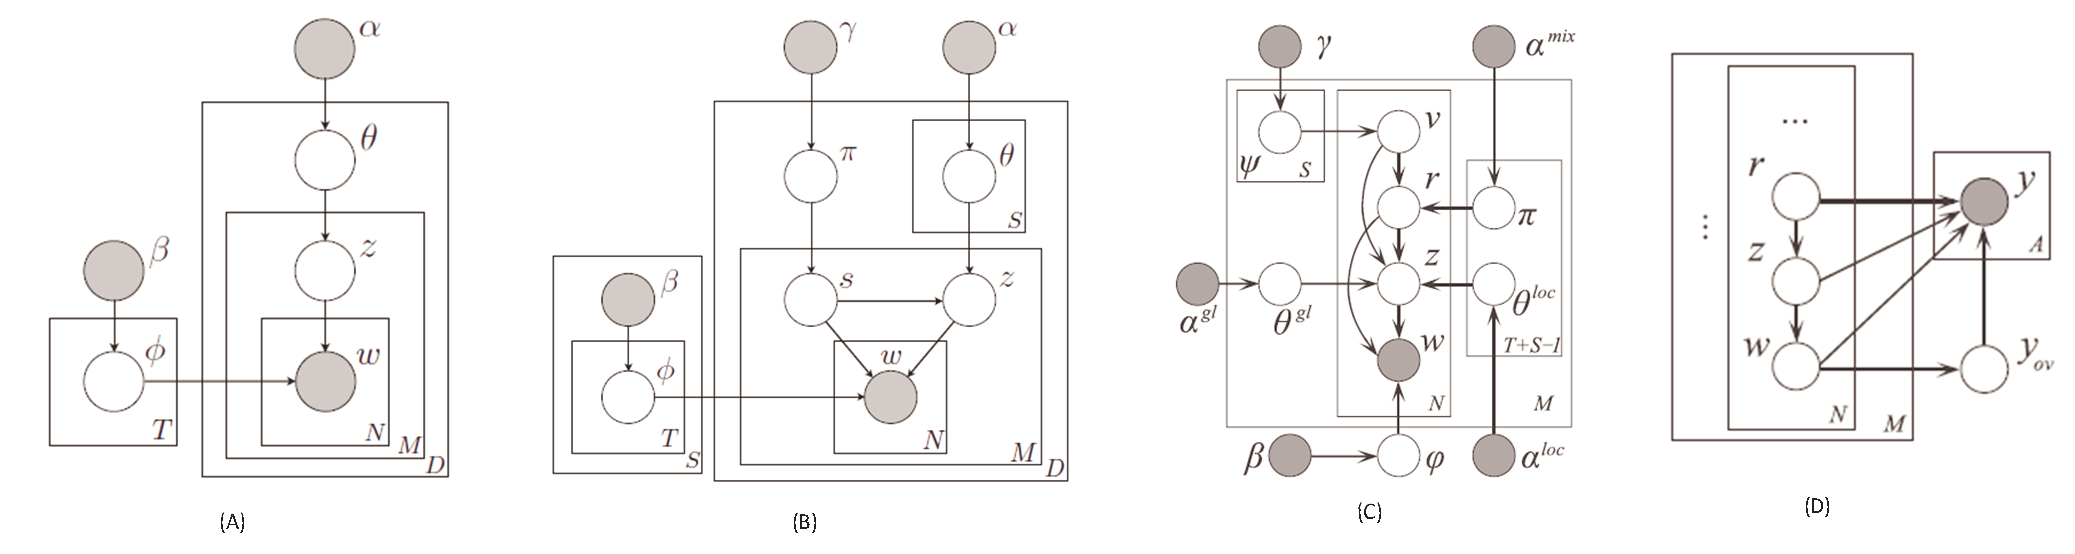
\includegraphics[scale=0.45]{figs/models.eps}
%	\caption{Different Bayesian networks: (A) Sentence-LDA for topic modelling
%	(B) Aspect and Sentiment Unification Model for sentiment analysis of reviews
%    (C) Multi-grained LDA model
%    (D) Multi-Aspect Sentiment model}
%	\label{fig:BNs}
%\end{figure*}


